%%%%%%%%%%%%%%%%%%%%%%%%%%%%%%%%%%%%%%%%%
% Simple Sectioned Essay Template
% LaTeX Template
%
% This template has been downloaded from:
% http://www.latextemplates.com
%
% Note:
% The \lipsum[#] commands throughout this template generate dummy text
% to fill the template out. These commands should all be removed when 
% writing essay content.
%
%%%%%%%%%%%%%%%%%%%%%%%%%%%%%%%%%%%%%%%%%

%----------------------------------------------------------------------------------------
%	PACKAGES AND OTHER DOCUMENT CONFIGURATIONS
%----------------------------------------------------------------------------------------

\documentclass[hidelinks, 12pt]{article} % Default font size is 12pt, it can be changed here

\usepackage{geometry} % Required to change the page size to A4
%\geometry{a4paper} % Set the page size to be A4 as opposed to the default US Letter

\usepackage{graphicx} % Required for including pictures
\usepackage{float} % Allows putting an [H] in \begin{figure} to specify the exact location of the figure
	\usepackage{wrapfig} % Allows in-line images such as the example fish picture
	\usepackage{setspace} % To control linespacing
	\usepackage{enumerate} % For enumerating lists
	\usepackage{enumitem} % more enumerating stuff
	\usepackage{multicol} % for multicoumn formating
	\usepackage{multirow} % for multicoumn formating
	\usepackage{adjustbox}
	\usepackage{changepage}
	\usepackage{fancyhdr}
	\usepackage[dvipsnames]{xcolor} %To change text colors, color options located at: http://en.wikibooks.org/wiki/LaTeX/Colors
	\usepackage[font={footnotesize}]{caption}
	\usepackage[labelfont=bf]{caption}
	\usepackage{longtable}
	\usepackage{tabularx}
	\usepackage{arydshln}
	\usepackage{titlesec} % To control section colors
	\usepackage{color}
	\usepackage[pdfencoding=auto, psdextra]{hyperref} % for web links
	\DeclareUnicodeCharacter{2212}{-}
	\DeclareUnicodeCharacter{2032}{'}
	
	\usepackage{soul}% for the underlining 
	\usepackage{frcursive}
	\usepackage{indentfirst}
	\usepackage{pdfpages}
	\usepackage{amsmath} % For other equations
	\usepackage{pgfplots} % For ploting graphs
	\pgfplotsset{width=15cm,compat=1.9}
	
	
	\graphicspath{{Pictures/}} % Specifies the directory where pictures are stored
	
	\linespread{1.2} % Line spacing
	\widowpenalty=8999 
	\clubpenalty=8999
	
	%Command for tabs
	\newcommand{\tab}{\hspace{20pt}}
	
	\usepackage[title]{appendix}
	\usepackage[toc, acronym, nopostdot, nonumberlist]{glossaries}
	\makeglossaries
\newacronym{vms}{VMS}{Viking Motorsports}
\newacronym{bms}{BMS}{Battery Management System}
\newacronym{ecu}{ECU}{Energy Control Unit}
	
	%%%%% Define PSU official colors
	\definecolor{PSUgreen}{RGB}{106,127,16}
	\definecolor{PSUltgreen}{RGB}{168,180,0}
	\definecolor{PSUblue}{RGB}{0,117,154}
	\definecolor{PSUltblue}{RGB}{161,216,224}
	\definecolor{PSUgray}{RGB}{71,67,52}
	\definecolor{PSUBrown}{RGB}{96,53,29}
	\definecolor{PSUsienna}{RGB}{163,63,31}
	\definecolor{PSUred}{RGB}{210,73,42}
	\definecolor{PSUorange}{RGB}{220,155,50}
	\definecolor{PSUyellow}{RGB}{230,220,143}
	\definecolor{PSUtan}{RGB}{232,221,162}
	\definecolor{PSUpurple}{RGB}{101,3,96}
	
	%----------------------------------------------------------------------------------------
	%  Section Colors
	%----------------------------------------------------------------------------------------
	\titleformat{\section}
	{\color{PSUgreen}\normalfont\Large\bfseries}
	{\color{PSUgreen}\thesection}{1em}{}
	
	\titleformat{\subsection}
	{\color{black}\normalfont\large\bfseries}
	{\color{black}\thesubsection}{1em}{}
	
	\titleformat{\subsubsection}
	{\color{PSUblue}\normalfont\normalsize\bfseries}
	{\color{PSUblue}\thesubsubsection}{1em}{}
	
	\titleformat{\subparagraph}
	{\color{PSUblue}\normalfont\normalsize\bfseries}
	{\color{PSUblue}\thesubsubsection}{1em}{}
	
	%----------------------------------------------------------------------------------------
	%  Watermark
	%----------------------------------------------------------------------------------------
	%\usepackage{draftwatermark} % for watermarks
	%\SetWatermarkText{\textbf{DRAFT}}
	%\SetWatermarkScale{5}
	%\SetWatermarkColor[gray]{0.9}
	%----------------------------------------------------------------------------------------
	\begin{document}
		\pagestyle{fancy}
		%----------------------------------------------------------------------------------------
		%	TITLE PAGE
		%----------------------------------------------------------------------------------------
		
		\begin{titlepage}
			\newcommand{\HRule}{\rule{\linewidth}{0.5mm}} % Defines a new command for the horizontal lines, change thickness here
			\center % Center everything on the page
			
			\HRule \\[0.4cm]
			{ \huge \color{PSUgreen}\bfseries Final Report for \texorpdfstring{\gls{bms}}{Battery Management System (BMS)} \\[0.4cm] \Large \emph{Sponsored by \texorpdfstring{\gls{vms}}{Viking Motorsports (VMS)}}}\\[0.4cm] % Title of your document
			\HRule \\[1.5cm]
			
			\textsc{\large Portland State University \\ Maseeh College of Engineering \& Computer Science \\ Department of Electrical \& Computer Engineering}\\[1.5cm]
			
			\begin{minipage}{0.4\textwidth}
				\large
				\emph{Authors:}\\
				Student1 \textsc{Jose Ramirez}\\
				Student2 \hspace{-3pt}\textsc{Hussein Khodor}\\
				Student3 \textsc{David Fransis}\\
				Student4 \hspace{-1pt}\textsc{Fangdong Yuan}\\
				{\large \today} % Date
				%{\large October 1, 2013} 
				%\includegraphics{Logo}\\[1cm] % Include a department/university logo - this will require the graphicx package
			\end{minipage}\\[0.5cm]
			\vfill % Fill the rest of the page with whitespace
			
\includegraphics[width=3.5in]{psuMCECSlogo_horiz.png}
			\vfill
			\textsc{\color{PSUgray}\normalsize ECE Capstone \\ Senior Project Development}\\[0.5cm] % Major heading such as course name
			
		\end{titlepage}
		
		%----------------------------------------------------------------------------------------
		%	Header
		%----------------------------------------------------------------------------------------
		\fancyhf{}  % clears the default page numbering
		\fancyhead[L]{\footnotesize{\textcolor{PSUgray}{Project Proposal}}}
		%\fancyhead[C]{\footnotesize{center head}}
		\fancyhead[R]{\footnotesize{\textcolor{PSUgray}{PSU ECE Capstone}}}
		%----------------------------------------------------------------------------------------
		%    Footer
		%----------------------------------------------------------------------------------------
		%\patchcmd{\footrule}{\hrule}{\color{PSUgreen}\hrule}{}{}
		\renewcommand{\footrulewidth}{0.4pt}
		\fancyfoot[L]{\footnotesize\color{PSUgray}\sffamily
			1930 SW 4$^{th}$ Ave, EB 102, Portland, OR 97201 \textbullet\ \href{https://www.pdx.edu/electrical-computer-engineering/}{www.pdx.edu/electrical-computer-engineering/}}
		%\fancyfoot[C]{~}
		\fancyfoot[R]{\footnotesize~\newline\color{PSUgray}\sffamily\thepage}
		
		%----------------------------------------------------------------------------------------
		%    TABLE OF CONTENTS
		%----------------------------------------------------------------------------------------
		\setcounter{tocdepth}{3}
		\tableofcontents % Include a table of contents
		%\setlength{\parskip}{3ex plus 2ex minus 2ex}
		
		%----------------------------------------------------------------------------------------
		%    Section: List of Figures & Tables
		%----------------------------------------------------------------------------------------
		\newpage
		\listoffigures
		%\newpage
		%\listoftables
		\pagebreak
		
		%----------------------------------------------------------------------------------------
		%   Section: Executive Summary
		%----------------------------------------------------------------------------------------
		\newpage
		\section{Executive Summary}
		\label{Executive_Summary}
		Our team will design the next-generation battery system for PSU’s electric Formula race car, EV27, in partnership with Viking Motorsports and our faculty advisor. The current EV program does not have a usable accumulator, so the car won’t run. Over the next two terms we will create a complete, competition-ready design for the high voltage battery pack and its Battery Management System (BMS), plus working low voltage prototype that demonstrates the core functions. The car we’re designing this battery for will compete in a Formula-style racing competition where universities bring their own cars to do a race competition.
		\pagebreak
		
		%----------------------------------------------------------------------------------------
		%   Section: Background and Research
		%----------------------------------------------------------------------------------------
		\newpage
		\section{Background}
		\label{Background}
		\gls{vms} is our sponsor. They are a medium-sized student group that participates in the Formula SAE Electric event.


Electric vehicles rely entirely on large battery packs as their primary energy source. These battery packs are made up of many individual cells, typically lithium-ion, that must operate within some strict electrical and thermal limits and requirements in order for them to remain safe, efficient, and long-lasting. Due to the fact that lithium-ion battery chemistry is sensitive to properties such as overcharging, over-discharging, overheating/temperature, and cell imbalance, electric vehicles often require a dedicated subsystem called the \gls{bms}, to monitor and protect the battery.

These systems exist because lithium-ion battery packs can be extremely dangerous if not carefully monitored and diagnosed. The individual cells can be damaged due to things such as overcharging, over-discharging, and overheating. So, electric vehicles incorporate a battery management system to act as a protective mechanism using a combination of sensing, diagnostics, and protective circuit logic within the system. The system ensures that the battery operates only within safe electrical and thermal limits, which can in turn improve safety, extend battery life, and optimize performance.

The battery management system continuously measures key parameters such as cell voltages, current flow, pack and cell temperatures, and the estimated state of charge. It then processes the data to compute additional metrics, such as pack health, state of energy, imbalance levels, and thermal stability. In addition to monitoring, the \gls{bms} controls balancing circuitry using techniques such as active or passive cell balancing, to keep individual cells at consistent charge levels. Additionally, the \gls{bms} manages protective actions such as overvoltage, undervoltage, and overcurrent cutoffs. Also, the \gls{bms} communicates diagnostic information, warnings, and operational status to the vehicle’s electronic control unit.

Within the larger electric vehicle system, the \gls{bms} serves as the central system responsible for determining whether the high-voltage battery pack is in a safe condition to deliver power to the vehicle. For instance, the electronic control unit depends on the \gls{bms} for accurate state of charge information, temperature status, and diagnostic reports. The motor, motor controller, charger, and thermal management system all rely on \gls{bms} outputs to function properly. Therefore, the \gls{bms} is not an isolated system but rather a core subsystem and safety component that interfaces with a lot of other components in the vehicle.

In practice, a battery management system is an electronic system that manages a rechargeable battery pack. Its operation follows a continuous loop of measure, protect, balance, and inform. First, it measures the fundamental state of the battery by using a network of sensors and integrated circuits to read the voltage of every individual cell, the total current flowing in or out of the pack, and its temperature at key locations. Second, it uses this data to protect the battery from damage by comparing the readings against safe limits. For instance, if it detects a dangerous condition like overvoltage, undervoltage, overcurrent, or extreme temperatures, it will command a safe shutdown by disconnecting the pack. Third, to maximize the pack’s capacity and longevity, it balances the cells, using techniques such as active or passive cell balancing to bleed off excess charge from higher voltage cells, ensuring all cells reach a uniform state of charge. Finally, it informs the larger system by processing the raw measurements into useful information such as state of charge and health, and it communicates this data, along with any warnings, to other devices.

According to the project description provided by Viking Motorsports, the electrical team has completed early conceptual research for the Formula SAE Electric platform. This foundational work includes preliminary investigation into CAN bus communication for vehicle subsystem networking, initial evaluation of cell monitoring integrated circuits and measurement topologies for per-cell voltage sensing, and high-level planning of the system-level safety architecture required to meet Formula SAE Electric fail-safe shutdown and interlock rules. These efforts established an initial understanding of the technical challenges and constraints associated with a high-voltage accumulator system but did not result in an implemented or tested \gls{bms} design.

At the start of this capstone project, no functional \gls{bms} hardware or firmware prototype exists, and there is no previous generation of a Viking Motorsports \gls{bms} to revise or extend. As a result, this project represents a ground-up design and development effort rather than an incremental revision. Our team is responsible for transforming the sponsor’s early conceptual research into a testable \gls{bms} prototype that performs real-time measurement, protection, balancing, and diagnostic functions that are suitable for future vehicle integration.

If nothing has been done on this project yet, are there comparable products or existing alternatives? Be creative here, what are similar technologies or direct competitors? Include them if they’re relevant or help describe your project.

See commercial off the shelf products and open source projects sections of the project proposal.

\subsection{Research}

\begin{figure}[H]
	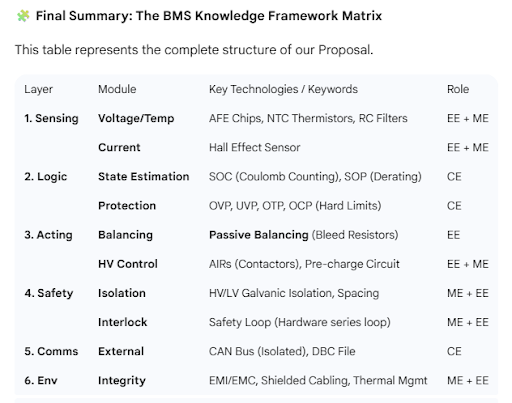
\includegraphics[width=0.75\linewidth]{research.png}
\end{figure}

\subsubsection{Commercial Off-the-Shelf Products}
Here are some options available to us for this project:

\begin{enumerate}
	\item \textbf{Orion \gls{bms} 2:} The Orion \gls{bms} 2 is a widely adopted \textbf{Centralized} solution in the FSAE and EV conversion sectors. While it integrates all measurement and control units into a single enclosure, offering mature reliability and EMI immunity, its architecture requires routing extensive sensing harnesses from all points of the battery pack to a central controller. This results in complex wiring and increased system weight. This serves as a critical counter-reference for our project: while centralized designs offer EMI advantages, their disadvantages in harness management within a high-voltage (300V+) and weight-critical racing environment validate our decision to pursue a Distributed Architecture.
	
	\item \textbf{Stafl Systems \gls{bms}1000M:} Stafl Systems utilizes a \textbf{Master-Slave Distributed Topology}. The system consists of a master controller (\gls{bms}1000M) and multiple satellite monitoring modules (\gls{bms}1101S), utilizing differential signaling (e.g., IsoSPI) for communication. This architecture significantly reduces the length of analog sensing wires, effectively lowering wiring complexity within the high-voltage pack. As a direct industry benchmark, Stafl demonstrates the engineering feasibility of distributed architectures for segmented packs. However, its Closed-Source nature limits secondary development for specific research algorithms, restricting its role to a hardware architecture reference.
	
	\item \textbf{EMUS G1 \gls{bms}:} EMUS G1 demonstrates a highly \textbf{Modular} distributed strategy, supporting the connection of multiple independent battery modules via CAN bus. This product employs robust galvanic isolation strategies and communication protocols ideal for physically separated battery enclosures (e.g., side-pod layouts). Given the potential requirement to split our 400V pack into multiple physical modules, EMUS provides a critical technical reference for High-Voltage Galvanic Isolation and data synchronization in our safety loop design.
\end{enumerate}

\subsubsection{Open Source Projects}
Here are some projects we can borrow from:

\begin{enumerate}
	\item \href{https://docs.fox\gls{bms}.org/}{fox\gls{bms} 2:} fox\gls{bms} 2 is a comprehensive, professionally developed open-source \gls{bms} platform from the Fraunhofer research institute, explicitly designed as a research and development platform for high-performance, high-availability battery systems. Its architecture is a master-slave distributed topology, where a central \gls{bms}-Master (ARM Cortex-R5) communicates via an interface board with daisy-chained Slave boards that handle cell monitoring (voltage/temperature) and passive balancing. The primary benefit is its exceptional depth. For instance, it offers a complete, well-documented hardware and software stack, including a built-in interlock line for safety shutdowns, CAN bus communication for system integration, and a flexible design that supports from a few cells up to several hundred kWh. The permissive licenses allow full use and modification. The notable drawback is its scale and complexity. For instance, as a generic research platform, it is not optimized for the strict space, weight, and FSAE-rule constraints of a race car. Its default use case is stationary storage, requiring significant adaptation for a mobile, high-vibration environment such as a race car. Nonetheless, it still serves as a great resource for robust system architecture, safety implementations such as interlock monitoring, and professional-grade, modular firmware structure.
	
	\item \href{https://libre.solar/\gls{bms}-c1/manual/}{Libre Solar \gls{bms}:} The Libre Solar \gls{bms} is a compact, fully integrated open-source \gls{bms} designed for stationary and small-scale mobile DC energy systems (12V-48V, up to 16 cells). Its architecture is highly centralized, combining the \gls{bms} Analog Front-End (Texas Instruments BQ76952), microcontroller (ESP32-C3), power MOSFETs, and communication interfaces (CAN, UART, I2C, USB, Bluetooth) on a single PCB. The primary benefit is its production-ready, all-in-one design that demonstrates efficient integration of core \gls{bms} functions such as cell monitoring, protection, passive balancing, and contactor control, within a minimal footprint. Its firmware, built on the Zephyr RTOS, provides a professional reference for implementing safety logic, the ThingSet protocol for configuration, and state-of-charge estimation. The notable drawback is its scale. For instance, it is designed for ~60V systems with currents up to 100A, its cell count and power handling are far below the requirements of a 400V+ FSAE powertrain. Its centralized architecture is also less ideal for the long, distributed battery pack typical in a race car frame. Nonetheless, it still serves as an excellent reference for PCB-level integration, component selection, and a clean, modular firmware structure that can inform the design of sub-modules within our larger, distributed system.
	
	\item \href{https://hackaday.io/project/181453-green-\gls{bms}}{Green \gls{bms}:} Green \gls{bms} is a hobbyist-developed, smart \gls{bms} designed for small-scale lithium battery packs such as for electric scooters or solar storage. Its architecture is a modular distributed system, using simple Cell Modules based on ATtiny microcontrollers to measure individual cell voltage/temperature, which report via I2C to a central Control Unit (Arduino Mega). The system includes a separate "Limiter" unit for contactor control and an Android app for monitoring. The primary benefit is its exceptional transparency and simplicity, it demonstrates the absolute core functions of a \gls{bms} (monitoring, protection, balancing) with minimal complexity, using widely understood components (Arduino, ATtiny). This makes it an excellent educational tool for understanding the fundamental data flow and logic of a \gls{bms} before engaging with more complex, integrated circuits. The significant drawbacks are its lack of automotive robustness, missing critical safety features (high-voltage isolation, CAN bus, fail-safe hardware interlocks), and limited scalability (I2C communication is unsuitable for long daisy-chains in a large pack). Nonetheless, it still serves as a valuable conceptual reference for system partitioning and basic 
\end{enumerate}

\subsubsection{Papers}
Here is some extra papers we read during our research:

\begin{enumerate}
	\item \href{https://web.archive.org/web/20200508032842id_/https://eprint.ncl.ac.uk/file_store/production/261931/F4ADEC30-2EDD-4881-A81A-AC0BFDE3D9EB.pdf}{Evaluation and Comparison of Battery Cell Balancing Methods:} This paper provides a structured, quantitative framework for selecting a cell balancing topology, directly addressing a key design decision. It categorizes and compares the three main balancing methods, dissipative (passive), capacitive energy transfer (active), and runtime balancing (active with converters), against critical metrics such as balancing speed, efficiency, complexity, and cost. This comparison is very valuable for our requirement to “support both active and passive cell balancing.” It provides an objective basis to decide whether to implement only passive (simpler, cheaper) or also include an active method (faster, more efficient) in our prototype.
	
	\item \href{https://ieeexplore.ieee.org/stamp/stamp.jsp?arnumber=8834858}{Review of Battery Cell Balancing Methodologies for Optimizing Battery Pack Performance in Electric Vehicles:} This paper provides a critical system-level perspective on cell balancing for batteries in electric vehicles, advocating for hybrid balancing methods that combine passive and active balancing techniques to leverage their respective advantages. This directly aligns with our requirement to “support both active and passive cell balancing,” suggesting an approach where both techniques work together in a complimentary manner (passive for continuous maintenance, active for rapid pre-charge equalization). Additionally, it highlights environmental factors, specifically operating temperature, thermal uniformity, and mechanical vibration, as crucial but under-researched variables that affect long-term balancing performance and cell degradation.
	
	\item \href{https://ieeexplore.ieee.org/stamp/stamp.jsp?arnumber=8320763}{State-of-the-Art and Energy Management System of Lithium-Ion Batteries in Electric Vehicle Applications: Issues and Recommendations:} This paper provides a holistic overview of Li-ion battery technology and the complete scope of a Battery Management System (\gls{bms}). It systematically covers core \gls{bms} functions critical to our project, such as cell condition monitoring, state estimation (SOC/SOH), charge/discharge control, protection circuitry, cell equalization, and thermal management. It is particularly valuable for understanding the interdependencies between different \gls{bms} subsystems and for identifying key challenges, such as managing temperature gradients and diagnosing faults, which are actively relevant to the harsh, high-vibration environment of a Formula SAE vehicle.
\end{enumerate}
		\pagebreak
		
		%----------------------------------------------------------------------------------------
		%   Section: Product Design Specification
		%----------------------------------------------------------------------------------------
		\newpage
		\section{Requirements}
		\label{Requirements}
		\subsection{Product Overview}
This paper provides a holistic overview of Li-ion battery technology and the complete scope of a \gls{bms}. It systematically covers core \gls{bms} functions critical to our project, such as cell condition monitoring, state estimation (SOC/SOH), charge/discharge control, protection circuitry, cell equalization, and thermal management. It is particularly valuable for understanding the interdependencies between different \gls{bms} subsystems and for identifying key challenges, such as managing temperature gradients and diagnosing faults, which are actively relevant to the harsh, high-vibration environment of a Formula SAE vehicle.

\subsection{Stackholders}
Our stakeholders include everyone who is directly or indirectly affected by the accumulator and \gls{bms} system. At the top level, we have our industry and university sponsors, who provide funding, facilities, and oversight, and care about safety, and reliability. The vehicle team are key users of our design: they integrate the pack into frame, rely on our interfaces, and depend on our documentation to build and service the system. Future student teams who will build, maintain, and possibly upgrade the pack are another important group, because our documentation will either make their work easier or harder.

\subsection{Requirements}

Must:
\begin{itemize}
	\item Continuously monitor all cell voltages and pack temperature.
	\item Provide reliable overvoltage, undervoltage, and overcurrent protection.
	\item Support both active and passive cell balancing.
	\item Communicate with the ECU over the CAN bus.
	\item Operate within SAE EV voltage limits and isolation standards.
	\item Include a fail-safe shutdown or interlock function for critical faults.
\end{itemize}

Should:
\begin{itemize}
	\item Include onboard data logging capability.
	\item Use modular architecture to scale for different battery pack sizes.
	\item Support self-diagnostic startup and fault recovery routines.
\end{itemize}

May:
\begin{itemize}
	\item Include an integrated display or diagnostic interface for local readings.
	\item Support wireless telemetry or USB debugging for testing.
\end{itemize}
		\pagebreak
		
		%----------------------------------------------------------------------------------------
		%   Section 4: Project Management Plan
		%----------------------------------------------------------------------------------------
		\newpage
		\section{Objectives and Deliverables}
		\label{Objectives and Deliverables}
		\subsection{Objectives}


\subsection{Deliverables}

Using the Atlassian suite of tools which include Jira, Bitbucket, and Confluence to deliver on the following

\begin{itemize}
	\item Project proposal
	\item Weekly Progress Reports
	\item Final report
	\item ECE Capstone Poster Session poster
	\item Detailed design documentation, explaining what your design does, how your design works, and why you made the decisions you did
	\item Electrical CAD: Schematics and board layouts, including output files (Gerbers, PDFs, etc)
	\item Mechanical CAD: enclosures, mechanisms, including output files (STLs, PDFs, etc)
	\item Bill of materials and pricing
	\item Developer's manual for future teams improveing on the existing design
	\item Short user manuals documenting how to use your creation
	\item A working prototype with a prototype battery pack and functionality with the \gls{ecu} prototype.
\end{itemize}
		\pagebreak
		
		%----------------------------------------------------------------------------------------
		%   Section 5: Signatures
		%----------------------------------------------------------------------------------------
		\newpage
		\section{Approach}
		\label{Approach}
		\input{Section_5}
		\pagebreak
		
		%----------------------------------------------------------------------------------------
		%   Section 6: Design
		%----------------------------------------------------------------------------------------
		\newpage
		\section{Design}
		\label{Design}
		\input{Section_6}
		\pagebreak
		
		%----------------------------------------------------------------------------------------
		%   Section 7: Test Plan Overview
		%----------------------------------------------------------------------------------------
		\newpage
		\section{Test Plan Overview}
		\label{Test Plan Overview}
		Our test plan consists of a top

We’re going to generate certain voltage and current values that qualify as Overvoltage, Undervoltage, and Overcurrent and the system will set the signal for the Shutdown Circuit and report each specific fault to the ECU with which specific cell(s) had the fault.

		\pagebreak
		
		%----------------------------------------------------------------------------------------
		%   Section 8: Results
		%----------------------------------------------------------------------------------------
		\newpage
		\section{Results}
		\label{Results}
		\input{Section_8}
		\pagebreak
		
		%----------------------------------------------------------------------------------------
		%   Section 9: Post Mortem
		%----------------------------------------------------------------------------------------
		\newpage
		\section{Post Mortem}
		\label{Post Mortem}
		\input{Section_9}
		\pagebreak
		
		%----------------------------------------------------------------------------------------
		%   Section 10: Future Work
		%----------------------------------------------------------------------------------------
		\newpage
		\section{Future Work}
		\label{Future Work}
		\input{Section_10}
		\pagebreak
		
		%----------------------------------------------------------------------------------------
		%   Section 11: Project Resources
		%----------------------------------------------------------------------------------------
		\newpage
		\section{Project Resources}
		\label{Project Resources}
		\input{Section_11}
		\pagebreak
		
		%----------------------------------------------------------------------------------------
		%   Section 12: Conclusion
		%----------------------------------------------------------------------------------------
		\newpage
		\section{Conclusion}
		\label{Conclusion}
		\input{Section_12}
		\pagebreak
		
		%----------------------------------------------------------------------------------------
		%    Section: Glossary
		%----------------------------------------------------------------------------------------
		\newpage
		\printglossary[type=\acronymtype]
		\pagebreak
		
		%----------------------------------------------------------------------------------------
		%   Section: Appendices
		%----------------------------------------------------------------------------------------
		\begin{appendices}
			%----------------------------------------------------------------------------------------
			%   Appendix A: Tooling
			%----------------------------------------------------------------------------------------
			\newpage
			\section{Tooling}
			\label{Tooling}
			\input{Appen_A}
			\pagebreak
			
			%----------------------------------------------------------------------------------------
			%   Appendix B: Developer’s Manual
			%----------------------------------------------------------------------------------------
			\newpage
			\section{Developer’s Manual}
			\label{Developer’s Manual}
			\input{Appen_B}
			\pagebreak
			
			%----------------------------------------------------------------------------------------
			%   Appendix C: User’s Manual
			%----------------------------------------------------------------------------------------
			\newpage
			\section{User’s Manual}
			\label{User’s Manual}
			\input{Appen_C}
			\pagebreak
			
			%----------------------------------------------------------------------------------------
			%   Appendix D: Test Plan
			%----------------------------------------------------------------------------------------
			\newpage
			\section{Test Plan}
			\label{Test Plan}
			\input{Appen_D}
			\pagebreak
		\end{appendices}
		
		
	\end{document}